\documentclass{article}

\usepackage{graphicx}
\usepackage[utf8]{inputenc}
\usepackage{fancyvrb}
\usepackage{amsmath}
\usepackage{booktabs}
\usepackage{float}
\usepackage{caption}
\usepackage{subcaption}
\usepackage{hyperref}
\usepackage{booktabs}   % for nicer tables
\usepackage{float}      % for [H] placement

\setlength{\parindent}{0pt}
% --- Packages ---
\usepackage[utf8]{inputenc}
\usepackage[english]{babel}
\usepackage{amsmath, amssymb} 
\usepackage{graphicx} 
\usepackage{fancyhdr}
\usepackage{xcolor}
\usepackage{booktabs}          
\usepackage{hyperref}          
\usepackage{geometry}
\usepackage{cite}
\addto\captionsenglish{\renewcommand{\bibname}{References}}
\geometry{
    a4paper,
    left=2cm,
    right=2cm,
    top=4cm,         % space for header
    bottom=2.5cm,      % space for footer
    headheight=3.7cm,
    headsep=0.8cm,
    footskip=1.2cm      % distance from bottom of text to baseline of footer
}
% Set up fancy header/footer
\pagestyle{fancy}
\fancyhf{}  % Clear all header/footer fields

% Header
\fancyhead[L]{
\includegraphics[height=2.3cm]{Figures/Logos/1.jpeg}}  % Left: Logo
\fancyhead[R]{\textbf{CRSBA}}  

% Footer
\fancyfoot[R]{Page \thepage}  

\renewcommand{\headrulewidth}{0.1pt} 
\renewcommand{\footrulewidth}{0.2pt} 
\renewcommand{\headrule}{\hbox to\headwidth{\color{lightgray}\leaders\hrule height \headrulewidth\hfill}} 
\renewcommand{\footrule}{\hbox to\headwidth{\color{lightgray}\leaders\hrule height \footrulewidth\hfill}}

\begin{document}

\section{Introduction}
In collaborative robotic tasks, achieving high-precision alignment for grasping objects is a significant challenge, particularly when the environment and arm cameras have different perspectives. This chapter details the development of a "Fine Control" layer for the AR4 robotic arm using Image-Based Visual Servoing (IBVS) and Homography-based mapping. Our approach utilizes a dual-camera system: a fixed global RealSense camera for initial brick detection and a local ESP32-CAM mounted on the end-effector for precise alignment. By bridging these two views with homography, we enable the robot to perform complex "Pick and Place" operations with high reliability and reduced computational overhead.

\section{Literature Review}
The development of this module was informed by several key research areas in robotic vision and control, focusing on robustness, multi-camera coordination, and non-conventional optics.

\subsection{Visual Servo Control Foundations}
Visual servoing is a robotic control technique that utilizes information from a vision sensor to regulate the pose (position and orientation) of a robot's end-effector relative to a target or environmental features \cite{Hutchinson1996}. It represents the fusion of results from multiple disciplines, including high-speed image processing, kinematics, dynamics, control theory, and real-time computing \cite{Hutchinson1996}. The fundamental objective is to create a closed-loop control system where visual information is used to minimize a vision-based error signal.

\subsection{The Pinhole Camera Model}
The foundation of visual servoing rests on the geometric mapping of 3D points in the environment onto a 2D image plane. As illustrated in Figure~\ref{fig:pinhole_model}, this process is modeled using the pinhole camera projection \cite{Hutchinson1996}.

\begin{figure}[H]
    \centering
    % Ensure you have uploaded the image as pinhole_model.jpg
    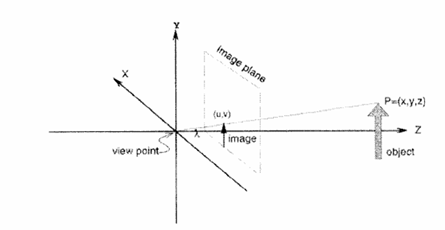
\includegraphics[width=0.6\textwidth]{Figures/VISP/pinhole_model.png}
    \caption{Perspective projection geometry showing the relationship between a 3D point $P$ and its 2D image projection $p$ \cite{Hutchinson1996}.}
    \label{fig:pinhole_model}
\end{figure}

For a 3D point $P = [X, Y, Z]^T$ in the camera frame $\{C\}$, its projection onto the image plane at coordinates $p = [x, y]^T$ is determined by the focal length $\lambda$ through similar triangles \cite{Hutchinson1996}:
\begin{equation}
    x = \lambda \frac{X}{Z}, \quad y = \lambda \frac{Y}{Z}
\end{equation}

This relationship is critical because it forms the starting point for the derivation of the \textbf{Interaction Matrix} (Image Jacobian). By differentiating these coordinates with respect to time, we can relate the velocity of image features $\dot{s}$ to the spatial velocity of the camera $v_c$ \cite{Hutchinson1996}.

\subsection{The Pinhole Camera Model}
The foundation of visual servoing rests on the geometric mapping of 3D points onto a 2D image plane. This process is modeled using the pinhole camera projection, where a 3D point $P = [X, Y, Z]^T$ in the camera frame $\{C\}$ is projected onto the image plane at coordinates $p = [x, y]^T$ via the focal length $\lambda$ \cite{Hutchinson1996}:
\begin{equation}
    x = \lambda \frac{X}{Z}, \quad y = \lambda \frac{Y}{Z}
\end{equation}
This projection is critical as it provides the geometric basis for the \textbf{Interaction Matrix} (Image Jacobian) used in the control law \cite{Hutchinson1996}.

\subsection{Position-Based Visual Servo (PBVS)}
In PBVS architectures, features extracted from image data are used in conjunction with a known geometric model of the target and camera parameters to estimate the target's pose relative to the camera frame \cite{Hutchinson1996}.



\subsubsection{Kinematic Error Function and Control Law}
A positioning task in PBVS is represented by a kinematic error function $E: \mathcal{T} \rightarrow \mathbb{R}^m$, where $\mathcal{T}$ is the task space of the robot \cite{Hutchinson1996}. The task is fulfilled when the end-effector is in a pose $x_e$ such that $E(x_e) = 0$. The regulator typically computes a desired end-effector velocity screw $u$ via:
\begin{equation}
    u = -k \hat{E}(x_e)
\end{equation}
where $k > 0$ is a proportional feedback gain and $\hat{E}$ is the estimated error based on reconstructed 3D geometry. The primary challenge remains the visual reconstruction problem, which is highly sensitive to camera calibration and robot kinematics.

\subsection{Image-Based Visual Servo (IBVS)}
IBVS defines the control task directly in the image feature space $\mathcal{F}$, avoiding the need for a full 3D interpretation of the scene \cite{Hutchinson1996}. The error signal is defined as $e(t) = f(t) - f_d$, where $f$ represents the current vector of image feature parameters and $f_d$ represents the desired feature configuration \cite{Hutchinson1996, Parisa2016}.



\subsubsection{The Image Jacobian (Interaction Matrix)}
The Image Jacobian $J_v$ is a linear transformation relating the rate of change in image feature parameters $\dot{f}$ to the camera's spatial velocity screw $\dot{r}$:
\begin{equation}
    \dot{f} = J_v(r)\dot{r}
\end{equation}



[Image of an Image Jacobian matrix equation]


For a 3D point $P = [x, y, z]^T$ under perspective projection with focal length $\lambda$, the velocity of its image plane coordinates $[u, v]^T$ relative to camera translational velocity $T$ and angular velocity $\Omega$ is:
\begin{equation}
    \begin{bmatrix} \dot{u} \\ \dot{v} \end{bmatrix} = \begin{bmatrix} \frac{\lambda}{z} & 0 & -\frac{u}{z} & -\frac{uv}{\lambda} & \frac{\lambda^2 + u^2}{\lambda} & -v \\ 0 & \frac{\lambda}{z} & -\frac{v}{z} & \frac{-\lambda^2 - v^2}{\lambda} & \frac{uv}{\lambda} & u \end{bmatrix} \begin{bmatrix} T_x \\ T_y \\ T_z \\ \omega_x \\ \omega_y \\ \omega_z \end{bmatrix}
\end{equation}
The manipulator velocity $u$ is then computed using the Moore-Penrose pseudoinverse $J_v^{+}$:
\begin{equation}
    u = -K J_v^{+}(r) e(f)
\end{equation}

\subsubsection{Advanced IBVS and Refined Frameworks}
Modern implementations utilize image moments $m_{ij}$ to describe complex shapes effectively, often combined with a \textbf{Coarse-to-Fine} framework for sub-millimeter accuracy \cite{Parisa2016, Bai2023}. This involves removing large initial alignment errors (15--30 cm) before using fine controllers to refine the pose within a 0.6 mm tolerance.

\subsection{Comparative Analysis: IBVS vs. PBVS}
The two primary paradigms in visual servoing differ in how they define the error signal and the space in which control is executed \cite{Hutchinson1996}.

\begin{figure}[H]
    \centering
    \begin{subfigure}[b]{0.48\textwidth}
        \centering
        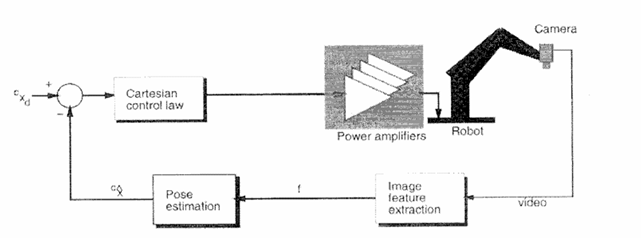
\includegraphics[width=\textwidth]{Figures/VISP/pbvs_diagram.png}
        \caption{Position-Based (PBVS) \cite{Hutchinson1996}}
    \end{subfigure}
    \hfill
    \begin{subfigure}[b]{0.48\textwidth}
        \centering
        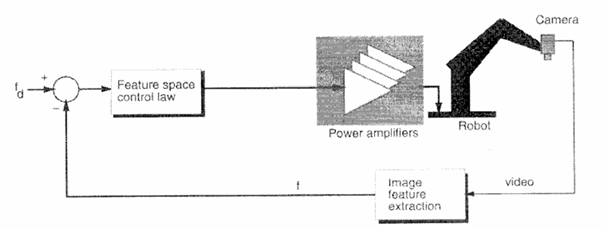
\includegraphics[width=\textwidth]{Figures/VISP/ibvs_diagram.png}
        \caption{Image-Based (IBVS) \cite{Hutchinson1996}}
    \end{subfigure}
    \caption{Control loop architectures. PBVS (left) relies on a 3D pose estimation block, while IBVS (right) regulates error directly in the image plane \cite{Hutchinson1996}.}
    \label{fig:vs_architectures}
\end{figure}

As illustrated in Figure~\ref{fig:vs_architectures}, PBVS is highly dependent on accurate 3D reconstruction, which introduces sensitivity to camera calibration errors \cite{Hutchinson1996}. In contrast, the IBVS approach regulates features directly in the image plane, making it inherently more robust to kinematic uncertainties and calibration biases \cite{Hutchinson1996}.

The selection of a visual servoing architecture involves critical trade-offs:
\begin{itemize}
    \item \textbf{Calibration Sensitivity:} IBVS is inherently less sensitive to camera calibration and robot kinematic errors compared to PBVS \cite{Hutchinson1996}.
    \item \textbf{Computational Complexity:} IBVS avoids nonlinear optimizations for 3D pose estimation but requires online computation of the depth-dependent Jacobian.
    \item \textbf{Stability:} IBVS can encounter singularities in the feature mapping function, while PBVS remains more intuitive for global stability in the Cartesian task space.
\end{itemize}

\subsection{Homography-Based Euclidean Reconstruction}
A significant advancement in bridging the gap between 2D features and 3D control is the use of Homography-based visual servoing. As established by Fang et al., a homography matrix $H$ relates the image coordinates of a target in a current view ($m_i$) to a desired reference view ($m_i^*$) through the relationship \cite{Fang2002}:
\begin{equation}
    m_i = H m_i^*
\end{equation}

\begin{figure}[H]
    \centering
    % Ensure the physical file is named exactly: homography_schematic.jpg
    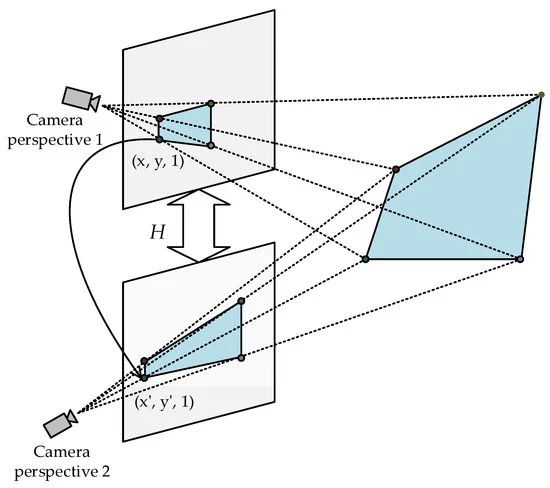
\includegraphics[width=0.4\textwidth]{Figures/VISP/homography_geometry.png}
    \caption{Schematic diagram of the planar homography transformation relationship between current and desired camera frames.\cite{MDPI2023}}
    \label{fig:homography_geometry}
\end{figure}



The homography matrix can be decomposed to achieve a Euclidean reconstruction of the scene. Specifically, $H$ is composed of the rotation $R$ and the translation $t$ between the two camera views, the normal vector $n^*$ of the object plane, and the distance $d^*$ from the reference camera to the plane \cite{Fang2002}:
\begin{equation}
    H = R + \frac{t}{d^*}n^{*T}
\end{equation}
This approach allows the system to recover the position and orientation of the robot relative to the target without requiring an explicit 3D model. In multi-camera systems, this enables the automation paradigm to shift from point-centric to scene-centric, effectively mapping coordinates observed in a global view (e.g., RealSense) into a local view (e.g., ESP32-CAM) to maintain asymptotic regulation of the end-effector \cite{Fang2002, Bai2023}.


\section{General Concept and Control Flow}
Visual servoing (VS) is a sensor-based control technique that utilizes real-time vision data as feedback to control the motion of a robot manipulator. In this project, visual servoing acts as the "Fine Control" layer, taking over after coarse global detection to ensure high-precision alignment.

The objective is to minimize an error vector $e(t) = s - s^*$, representing the difference between current visual features ($s$) and desired features ($s^*$). The system follows a structured flow: perception of local corners via the eye-in-hand camera, target feature generation, error calculation, and the transformation of image-plane errors into Cartesian velocity commands.

\begin{figure}[H]
    \centering
    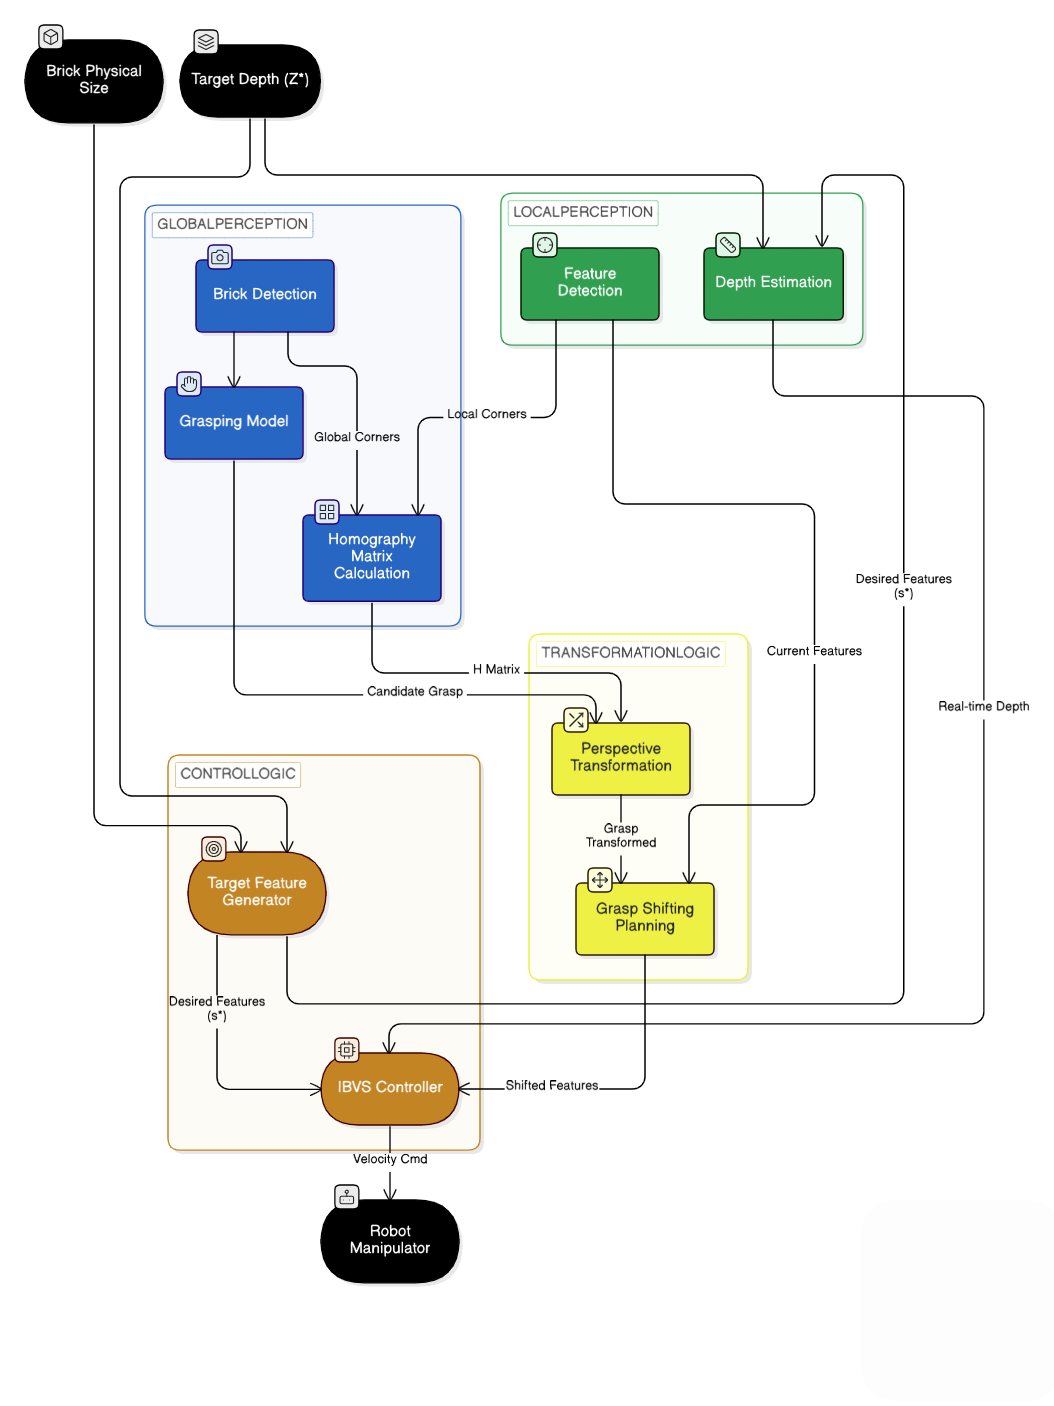
\includegraphics[width=0.6\textwidth]{Figures/VISP/VisualServoDiagram.png}
    \caption{System Architecture Flowchart: Integration of Global Perception and Local IBVS Control.}
    \label{fig:flow_diagram}
\end{figure}

\section{Implementation Details}

The implementation of the fine-control layer is structured into modular functional blocks that facilitate the transition from global environmental perception to high-precision local manipulation.

\subsection{Local Perception and Depth Estimation}
The local perception block provides high-frequency feedback for the closed-loop controller.
\begin{itemize}
    \item \textbf{Feature Detection:} A Region of Interest (ROI) tracker is employed to minimize computational load. It utilizes HSV color-space thresholding to isolate the brick and applies a fisheye distortion model to undistort coordinates . The tracker is initialized by the ``seed'' point provided by the transformation logic to ensure it locks onto the correct target .
    \item \textbf{Depth Estimation:} Real-time depth ($Z_{curr}$) is estimated by comparing the pixel area of the current features ($Area_{curr}$) to the dynamically calculated target area ($Area_{target}$). The system applies a smoothed area projection law :
    \begin{equation}
        Z_{curr} = Z_{target} \cdot \sqrt{\frac{Area_{target}}{Area_{curr}}}
    \end{equation}
\end{itemize}

\subsection{Global Perception and Homography Matrix Calculation}
The system initiates coordination by bridging the heterogeneous perspectives of the Realsense environment and ESP32 arm cameras. 
\begin{itemize}
    \item \textbf{Brick Detection and Grasping Model:} The environment camera identifies candidate targets and computes a candidate grasp point $(u, v , z) $where $u$ , $v$  represents the grasp points pixel coordinates and $z$ represents the orientation angle .
    \item \textbf{Geometric Feature Matching:} To ensure cross-camera consistency, the system extracts rotated bounding box corners and calculates the length-to-width ratio of the detected brick. A candidate is only validated if its aspect ratio matches the local view within a 20\% tolerance .
    \item \textbf{Homography Estimation:} Once a match is confirmed, a Homography matrix $H$ is computed using the RANSAC algorithm. This matrix serves as the mathematical bridge to relate current image coordinates $m_i$ to reference coordinates $m_i^*$ via $m_i = H m_i^*$ .
\end{itemize}

\subsection{Transformation Logic}
This block translates global strategic goals into local tactical coordinates for the end-effector.
\begin{itemize}
    \item \textbf{Perspective Transformation:} The candidate grasp point is projected into the local camera's image plane using the calculated matrix $H$. While the $U$ and $V$ pixel coordinates are transformed to account for the perspective shift, the orientation angle ($Z$) is passed directly to stabilize the goal state .
    \item \textbf{Grasp Shifting Planning:} The system ``latches'' onto the initial transformed point to set a local reference. It calculates a shift vector between the current brick centroid and the desired grasp pixel, effectively shifting the target features so the controller aligns the gripper with the specific grasp point rather than the brick center .
\end{itemize}

\subsection{Control Logic and Feature Generation}
The final stage generates the desired goal state and executes the motion command.
\begin{itemize}
    \item \textbf{Target Feature Generator:} The system defines the desired state $s^*$ by projecting a virtual 3D model of the brick into the image plane. It implements ``Snap-to-Grid'' logic to round the grasp angle to the nearest $90^\circ$, preventing rotational oscillations during the approach .
    \item \textbf{IBVS Controller:} The Image-Based Visual Servoing (IBVS) controller minimizes the error $e(t) = s - s^*$. It utilizes the Image Jacobian ($L$) to translate pixel errors into 6-DOF velocity commands, enabling the robot manipulator to achieve sub-millimeter alignment for the final pick operation .
\end{itemize}
\section{Results and Evaluation}
Experimental trials focused on stability and convergence. The pixel error norm successfully converged to $< 5$ pixels. The inclusion of RANSAC ensured sensor noise did not break the tracking lock, and fisheye calibration significantly reduced systematic bias.

\begin{thebibliography}{99}
\bibitem{Hutchinson1996} S. Hutchinson, G. D. Hager, and P. I. Corke, "A Tutorial on Visual Servo Control," \textit{IEEE Transactions on Robotics and Automation}, vol. 12, no. 5, pp. 651-670, 1996.
\bibitem{Fang2002} Y. Fang, D. M. Dawson, W. E. Dixon, and M. S. de Queiroz, "Homography-Based Visual Servoing of Wheeled Mobile Robots," \textit{Proc. 41st IEEE Conf. Decision and Control}, 2002.
\bibitem{Parisa2016} P. M. Khiabani, et al., "Visual Servoing Simulator by Using ROS and Gazebo," \textit{4th Int. Conf. on Robotics and Mechatronics (ICRoM)}, 2016.
\bibitem{Bai2023} Y. Bai, et al., "EA-CTFVS: An Environment-Agnostic Coarse-to-Fine Visual Servoing Method for Sub-Millimeter-Accurate Assembly," \textit{Actuators}, vol. 12, no. 1, 2023.
\bibitem{MDPI2023} A. G. Schiano, et al., "A Review of Homography Estimation: Advances and Challenges," \textit{MDPI: Sensors}, vol. 23, 2023.
\end{thebibliography}
\end{document}